Bijels require a multiscale modeling approach to accurately capture the rich array of physical phenomena 
occurring across multiple length and time scales. Within a bijel, one must consider fluid flow, phase separation, particle-fluid coupling, and interparticle 
interactions. The characteristic length scales span from nanometers to micrometers, demanding a model capable of resolving fine structural details while also 
capturing mesoscale dynamics. In the following sections, a comprehensive review of the relevant physical processes is provided, laying the foundation for the 
numerical methods used in this work.

\section{Hydrodynamics}

Mass conservation is derived by applying the conservation principle to a differential control volume, which characterizes the mass flux through its boundaries. Assuming no sources or sinks of mass, the conservation equation takes the form of the continuity equation:

\begin{equation}
    \frac{\partial\rho}{\partial t} + \nabla\cdot\left(\rho\vec{u}\right) = 0
\end{equation}

where $\rho$ is the fluid density and $\vec{u}$ is the velocity vector field.
Momentum conservation can be obtained by applying Newton's second law to the fluid element. This yields the momentum balance equation, where changes in momentum arise due to pressure gradients, 
viscous stresses, and body forces. The general form of the momentum equation is:

\begin{equation}
    \rho \left(\frac{\partial\vec{u}}{\partial t} + (\vec{u}\cdot\nabla)\vec{u} \right) = -\nabla p + \nabla \cdot \boldsymbol{\tau} + \vec{f}
\end{equation}

where $p$ is the pressure field, $\boldsymbol{\tau}$ is the viscous stress tensor, and $\vec{f}$ represents body forces such as gravity or magnetic interactions.

For a Newtonian, isotropic fluid, the viscous stress tensor is defined as:

\begin{equation}
    \boldsymbol{\tau} = p\mathbf{I} + \eta\left( \nabla \vec{u} + (\nabla \vec{u})^T \right) - \frac{2}{3}\eta(\nabla \cdot \vec{u})\mathbf{I}
\end{equation}

where $\eta$ is the dynamic viscosity. The pressure term can be related to the bulk viscosity $\lambda$ as

\begin{equation}
    p = \left( \lambda + \frac{2}{3}\eta \right) \nabla \cdot \vec{u}
\end{equation}

Substituting this stress tensor into the momentum equation yields the compressible Navier-Stokes equation,

\begin{equation}
    \rho \left(\frac{\partial\vec{u}}{\partial t} + (\vec{u}\cdot\nabla)\vec{u} \right) = -\nabla p + \eta \Delta \vec{u} + \frac{1}{3}\eta \nabla(\nabla \cdot \vec{u}) + \vec{f}
\end{equation}

For an incompressible fluid, meaning that the constant density and negligible bulk viscosity, the condition $\nabla \cdot \vec{u} = 0$ holds. Under this 
assumption, the Navier-Stokes equation simplifies to,

\begin{equation}
    \rho \left(\frac{\partial\vec{u}}{\partial t} + (\vec{u}\cdot\nabla)\vec{u} \right) = -\nabla p + \eta \Delta \vec{u} + \vec{f}
\end{equation}

As there are no external forces like gravity acting on the fluid and there are is no hydrodynamic pressure being applied to the fluid, $-\nabla p = \vec{f} = 0$ resulting in the
following form of the incompressible Navier Stokes equation.

\begin{equation}
    \rho \left(\frac{\partial\vec{u}}{\partial t} + (\vec{u}\cdot\nabla)\vec{u} \right) = \eta \Delta \vec{u}
\end{equation}

To facilitate numerical simulation and analysis, it is often useful to express the Navier-Stokes equation in non-dimensional form. Introducing characteristic scales for length 
$l_0$, time $t_0$, and density $\rho_0$, dimensionless variables are defined as

\begin{equation}
    \bar{l} = \frac{l}{l_0}, \quad \bar{t} = \frac{t}{t_0}, \quad \bar{\rho} = \frac{\rho}{\rho_0}
\end{equation}

Substituting these into the incompressible Navier-Stokes equation leads to the dimensionless form:

\begin{equation}
    \frac{\partial \bar{\vec{u}}}{\partial \bar{t}} + (\bar{\vec{u}} \cdot\nabla)\bar{\vec{u}} = \frac{1}{Re} \Delta \bar{\vec{u}}
\end{equation}

where the Reynolds number is defined as $Re = \frac{\rho_0 u_0 l_0}{\eta}$ which characterizes the ratio of inertial to viscous forces in the system.

\section{Phase separation}

Bijels form through spinodal decomposition of two partially miscible fluids, a process that can be effectively modeled using the Cahn-Hilliard equation, which describes the diffusive dynamics 
of a conserved scalar order parameter $\phi$, typically representing the local concentration difference between the two fluid components,

\begin{equation}
    \frac{\partial \phi}{\partial t} = \nabla \cdot \left( M \nabla \mu \right)
\end{equation}

Here, $M$ is the mobility coefficient and $\mu$ is the chemical potential, which is derived from the variation of the free energy functional $F[\phi]$. This formulation allows for the modeling of 
interfacial tension and the spontaneous formation of bicontinuous domains characteristic of spinodal decomposition.
To capture not only the diffusive separation of phases but also the resulting fluid motion, the Cahn-Hilliard equation is coupled with the Navie-Stokes equations, leading to the 
Cahn-Hilliard-Navier-Stokes (CHNS) framework. This coupling is essential in systems like bijels, where hydrodynamic interactions play a significant role in domain coarsening and morphology arrest. 
The momentum conservation equation in this framework is written as:

\begin{equation}
    \rho \left(\frac{\partial\vec{u}}{\partial t} + (\vec{u}\cdot\nabla)\vec{u} \right) = \eta \Delta \vec{u} + \nabla \cdot P_{\text{therm}}
\end{equation}

Here, $\vec{u}$ is the velocity field, $\rho$ is the fluid density, and $\eta$ is the dynamic viscosity. The term $P_{\text{therm}}$ represents the thermodynamic pressure tensor, which incorporates 
contributions from gradients in the order parameter and is directly linked to the chemical potential \(\mu\). This tensor encodes the capillary and interfacial forces arising from phase separation 
and effectively couples the compositional dynamics to the fluid flow.
The CHNS model enables simulation of complex phase-separating fluid systems, capturing both the interfacial evolution and the momentum transfer within the fluid. In the context of bijels, this 
model can be used to predict the formation and stabilization of the bicontinuous structure, especially when interfacial jamming by colloidal particles is introduced in more advanced extensions.

\section{Particle dynamics}

In computational studies of particle-laden fluids, particles can be modeled either as point particles or as explicitly resolved rigid bodies. The choice between 
these approaches depends on the physical fidelity required, the computational cost, and the scales at which particle-fluid and particle-interface interactions must be resolved.

Point particle models treat colloids as infinitesimal entities that influence the surrounding fields through source terms or effective force laws. 
\cite{mehrabadi_direct_2018, prosperetti_point-particle_2007, frohlich_validation_2018}
In such models, 
particles do not occupy physical volume and their influence on the fluid is typically introduced via body forces or perturbations to the chemical potential field. This 
approach is computationally efficient and particularly useful for systems with a large number of particles or when only large-scale collective behavior is of interest. 
However, point particles cannot capture rotational dynamics, or hydrodynamic effects such as lubrication forces. Additionally, 
their interaction with phase interfaces is often prescribed rather than emergent, limiting their accuracy in systems like bijels where particles jam at fluid-fluid interfaces 
and significantly modify the interface topology.

In contrast, explicit particle models represent colloids as finite-size rigid bodies with well-defined shape, volume, and surface boundary conditions. 
\cite{ladd_numerical_1994, jansen_bijels_2011,gunther_timescales_2014}
These particles interact 
with the surrounding fluid through no-slip or slip boundary conditions, and their motion responds dynamically to hydrodynamic, capillary, and interparticle forces. By resolving 
particle geometry, these models allow for accurate representation of rotational motion, surface wetting and interfacial adsorption.
\cite{jansen_bijels_2011, gunther_lattice_2013}
This is important in bijel systems, where particle-induced jamming depend on particle shape, size, and surface wetting. 

An intermediate approach between point particles and explicitly resolved rigid bodies is the immersed boundary method (IBM), which represents extended particles as collections of 
point markers embedded in the fluid. \cite{peskin_immersed_2002, luo_immersed-boundary_2008, spandan_parallel_2017}
These markers interact with the fluid through momentum exchange that impose motion onto the surrounding fluid, effectively reconstructing 
the dynamics of a deformable or rigid object without requiring an explicit boundary mesh. \cite{peskin_immersed_2002, luo_immersed-boundary_2008, spandan_parallel_2017} 
IBM has been widely used in biological and colloidal systems, to model the dynamics of deformable bodies. \cite{peskin_immersed_2002, luo_immersed-boundary_2008, spandan_parallel_2017}

For systems in which interfacial structure, jamming, or near-field hydrodynamics play a central role as in bijel formation, explicit particle modeling 
is generally preferred as we are able to resolve the interfacial structure and near field hydrodynamics without the complications of IBM.

\section{Magnetic fields and particles}

% The Shan-Chen pseudopotential
% model is used to simulate the Cahn-Hilliard equation, defined below

% \begin{equation}
%     \begin{split}
%     \frac{\partial\phi}{\partial t}+\nabla\cdot\left(\phi\vec{u}\right) &= \nabla \cdot \left( \Gamma  \nabla\phi \right)
%     \end{split}
% \end{equation}

% where $c^k$, $M^k$ and $u^k$ is the concentration, mobility and velocity of species $k$ respectively while $\mu$ is the free energy of system. 
% \cite{shan_lattice_1993, shan_simulation_1994, he_lattice_1997, he_discrete_1998}



% A computational model designed to simulate soft matter systems 
% at the mesoscale must accurately represent both hydrodynamics and non-ideal mixing in order to capture the essential physics of emulsions, colloids, and phase-separating fluids. 
% A hydrodynamic model must be able to recover mass and momentum conservation of a incompressible fluid

% Modelling multicomponent dynamics requires incorporating a free energy model between fluids, allowing for the implementation of
% chemical potential driven mass transfer and surface tension. Typically this is done using a Cahn-Hilliard model based on a
% square gradient free energy functional. This captures the demixing characteristics of phase separating fluids and controls interface
% characteristics, providing surface tension and interface width characteristics. This model has been used in past investigations looking 
% into spinodal decomposition, domain growth and coarsening. 


% To fully capture mesoscale dynamics, the model must also resolve the coupling between hydrodynamic flow and composition gradients. This coupling 
% is essential for simulating phenomena such as Marangoni flows, interfacial instabilities, and anisotropic stress distributions that arise from 
% non-uniform compositions or curvature-dependent surface tension. Moreover, the model must support anisotropic or time-dependent external fields 
% (e.g., magnetic, electric, or shear) that influence mixing behavior. Computational frameworks that can evolve velocity, pressure, and composition 
% fields simultaneously—while ensuring thermodynamic consistency and mechanical stability—are critical for accurately describing the emergent structures 
% and transport properties in non-ideal soft matter systems.

% Given the multiscale modeling necessary to correctly simulate the physical system, one approach suggested to tackle this problem is the multicomponent
% Lattice Boltzmann Method. This technique bridges the length and time scales necessary in soft matter modeling through modeling the evolution of a particle
% distribution function. Hydrodynamic parameters are recovered through calculating the moments of the particle distribution function. One of the advantages of
% the Lattice Boltzmann Method its parallelize nature and ease of adding multiple physical phenomena. In the following sections, the implementation of the LBM
% and alternatives to the LBM will be presented.

% This work uses a multicomponent Lattice Boltzmann Method (LBM) to simulate the hydrodynamics of two partially miscible, 
% incompressible fluids as implemented in LB3D. The LBM solves the continuity and Navier-Stokes equation at low
% Mach and Reynolds numbers for the fluid, defined as, 

% \begin{equation}
%     \begin{split}
%     \frac{\partial\rho}{\partial t} + \nabla\cdot\left(\rho\vec{u}\right) &= 0 , \\
%     \frac{\partial\vec{u}}{\partial t} + (\vec{u}\cdot\nabla)\vec{u} &= - \frac{1}{\rho} \nabla p + \nu \nabla^2 \vec{u} ,
%     \end{split}
% \end{equation}

% incorporating density $(\rho)$, viscosity $(\eta)$, velocity $(u)$, pressure $(P)$, and 
% body force $(F_{body})$. \cite{qian_lattice_1992, chin_lattice_2002, nourgaliev_lattice_2003} The Shan-Chen pseudopotential
% model is used to simulate the Cahn-Hilliard equation, defined below

% \begin{equation}
%     \begin{split}
%     \frac{\partial\phi}{\partial t}+\nabla\cdot\left(\phi\vec{u}\right) &= \nabla \cdot \left( \Gamma  \nabla\phi \right)
%     \end{split}
% \end{equation}

% where $c^k$, $M^k$ and $u^k$ is the concentration, mobility and velocity of species $k$ respectively while $\mu$ is the free energy of system. 
% \cite{shan_lattice_1993, shan_simulation_1994, he_lattice_1997, he_discrete_1998}

% Particle dynamics include Hertzian contact and lubrication forces, tracked with classical Newtonian mechanics, while 
% particle-fluid coupling involves momentum exchange to simulate viscous dissipation. Particle-particle magnetic interactions are modeled using dipole 
% interactions. \cite{davies_interface_2014, xie_direct_2017, xie_controllable_2021} A more detailed description of the model is 
% provided in the following sections

Magnetically responsive particles can generally be classified as paramagnetic or ferromagnetic, depending on the nature and strength of their magnetization in response to external 
magnetic fields. Paramagnetic particles do not possess a permanent magnetic moment but acquire a reversible magnetization that aligns with the applied field and 
vanishes once the field is removed. \cite{sinn_magnetically_2011} Their response is typically linear with field strength and does not involve magnetic hysteresis. 
In contrast, ferromagnetic particles exhibit strong, permanent magnetization due to the alignment of magnetic domains even in the absence of an external field. These particles can 
exhibit hysteresis and significantly stronger dipole-dipole interactions. \cite{sinn_magnetically_2011}
As a result, ferromagnetic particles are more likely to form irreversible aggregates or chains, while paramagnetic particles 
respond more gently and reversibly, making them preferable in systems where tunability and field-off stability are important. The choice between these types depends on the desired 
degree of responsiveness, reversibility, and control in applications such as field-directed assembly or responsive emulsions.

Magnetic particles are often modeled using the magnetic dipole approximation, which treats each particle as possessing a single point dipole moment \(\vec{m}\) located at its center.
\cite{davies_assembling_2014}
The dipole-dipole interaction between two particles separated by a vector \(\vec{r}\) is described by the potential:

\begin{equation}
    U_{\text{d}} = \frac{\mu_0}{4\pi r^3} \left[ \vec{m}_1 \cdot \vec{m}_2 - 3(\vec{m}_1 \cdot \hat{r})(\vec{m}_2 \cdot \hat{r}) \right]
\end{equation}

This model captures the long-range, anisotropic nature of magnetic interactions and is commonly used due to its simplicity and computational efficiency. It is especially effective when 
particles are small, well-separated, and uniformly magnetized, such that higher-order multipole contributions can be neglected. However, the dipole model becomes less accurate when particles 
aggregate closely or experience strong magnetic fields that cause internal magnetization to deviate from a uniform state.

To address these limitations, the demagnetization tensor method offers a more refined model by considering the particle as a uniformly magnetized ellipsoid and calculating the internal magnetic 
field using an analytical or numerically tabulated demagnetization tensor. \cite{takahashi_ellipsoids_2017} 
This method accounts for the effect of particle shape on the distribution of internal magnetization and enables the modeling of induced magnetic 
dipoles that respond to local fields. The total magnetic field of an ellipsoids can be written,

\begin{equation}
    \mathbf{H}(r) = \mathbf{H}_0 + \mathbf{N}(r)\mathbf{K}\mathbf{H}^{\dagger}
\end{equation}

Where $\mathbf{H}(r)$ is the total magnetic field of the ellipsoids, $\mathbf{H}_0$ is the inducing magnetic field in each direction,
$\mathbf{K}$ is the susceptibility tensor and $\mathbf{H}^{\dagger}$ is the resultant uniform magnetic field at any point within
the ellipsoids. \cite{takahashi_ellipsoids_2017}  This approach is particularly useful for modeling spheroidal or ellipsoidal particles and is widely 
used in magnetorheological systems, chain-forming ferrofluids, and dense suspensions where particle-particle interactions are shape-dependent.

Since bijel formation and stabilization primarily depend on interfacial 
jamming and long-range interactions between particles at fluid-fluid interfaces, the magnetic dipole approximation is often sufficient to model key behaviors such as chaining, orientation under external 
fields, and capillary-mediated assembly. However, if particle shape anisotropy, proximity effects, or induced magnetization in response to local fields are important, incorporating demagnetization tensors 
may offer improved realism.

\section{Numerical modeling}

\subsection{Multiscale modeling algorithms}

A wide range of numerical methods exist for simulating the physics details in previous sections. The choice of method depends on the specific physical processes to be captured such as 
interface dynamics, hydrodynamic interactions, and thermal fluctuations—as well as computational efficiency and scalability. Below, we outline several commonly used approaches that have been 
applied in studies of complex fluids and soft matter systems.

The Volume of Fluid (VOF) method is a sharp-interface technique used to track the evolution of fluid-fluid interfaces within a fixed computational grid 
\cite{gopala_volume_2008, fleckenstein_volume-fluid-based_2015, deising_direct_2018}. In VOF, a scalar field representing the volume fraction of one 
fluid is defined for each grid cell to indicate the local phase composition. Interface reconstruction algorithms are then employed to geometrically 
localize the boundary between phases. The method is inherently mass-conserving and can handle large interface deformations, making it particularly 
effective for high-Reynolds-number flows and surface-tension-driven phenomena. However, VOF methods can struggle with accurately capturing interfacial 
curvature and are not well-suited for diffuse interfaces, which limits their applicability in modeling spinodal decomposition and phase separation 
processes such as those that form bijels.

Phase field methods use a diffuse-interface approach to model multiphase systems, representing fluid composition or phase identity through a continuous 
order parameter field governed by equations such as the Cahn-Hilliard or Allen-Cahn equations 
\cite{mendoza_evolution_2006, carmack_tuning_2018, chan_channel_2012}. These methods naturally capture smooth transitions between phases, enable
accurate computation of interfacial forces, and handle topological changes like coalescence and breakup with ease. Derived from variational principles, 
phase field models are thermodynamically consistent, making them particularly well-suited for simulating spinodal decomposition, wetting phenomena, and 
interfacial dynamics. However, their main limitations include the need for fine spatial resolution near interfaces to maintain accuracy and the relatively 
high computational cost of solving fourth-order PDEs, especially when coupled with full hydrodynamic models.

Brownian dynamics is a particle-based simulation method used to model the stochastic motion of colloidal particles suspended in a fluid 
\cite{huber_brownian_2019, yip_brownian_2005, elsawy_utility_2025}. It approximates the over-damped limit of Langevin dynamics by integrating 
particle trajectories under the influence of both deterministic forces—such as interparticle potentials or external fields—and random thermal 
forces representing collisions with solvent molecules. Hydrodynamic interactions may be included through approximate mobility tensors or omitted 
entirely, depending on the desired level of fidelity. Brownian dynamics is particularly well-suited for studying self-assembly, aggregation, and 
diffusion in dilute suspensions, where particle motion is dominated by thermal fluctuations. However, it does not model the surrounding fluid 
explicitly, limiting its ability to capture bulk fluid flow or interface-mediated interactions. As a result, Brownian dynamics is not sufficient 
on its own for simulating the coupled fluid-particle dynamics involved in bijel formation.

The Lattice Boltzmann Method (LBM) is a discretization of the Boltzmann equation of motion for molecules. \cite{qian_lattice_1992, succi_lattice_2018, shan_multicomponent_1995, swift_lattice_1996}
Unlike traditional CFD techniques such as phase field or VOF methods, LBM tracks the evolution of a 
particle distribution function within grid cells evolved through a discretized Boltzmann equation of motion. Macroscopic variables such as fluid density and 
velocity are recovered from the particle distributions through appropriate moment integration, and the Navier Stokes equation at the incompressible limit can be 
obtained through a Chapman-Enskog expansion of the LBM. \cite{qian_lattice_1992} The LBM has become an attractive tool for meso-scale CFD simulations due to its ease of algorithm 
implementation, highly parallelizable nature and ease of boundary condition implementation, allowing coupling to other physically relevant systems such as 
particles with varieties of potentials, external fields and deformable bodies.

The particle distribution function described earlier is advected on a pre-constructed lattice stencil, commonly denoted as DnQm where n and m represent the 
number of dimensions and directions in the stencil. \cite{succi_lattice_2018, schmieschek_lb3d_2017}
Common stencils include the D1Q5, D2Q9 and D3Q19 stencil, all of which recover mass and momentum conservation. 
For energy conservation, a higher order stencil such as D3Q27 is necessary. The D2Q9 and D3Q19 stencils have 9 and 19 populations respectively that include 
connections to nearest and next nearest neighbour points. The D3Q19 stencil is shown in Figure \ref{fig:d3q19_lattice}.

\begin{figure}[h]
    \centering
    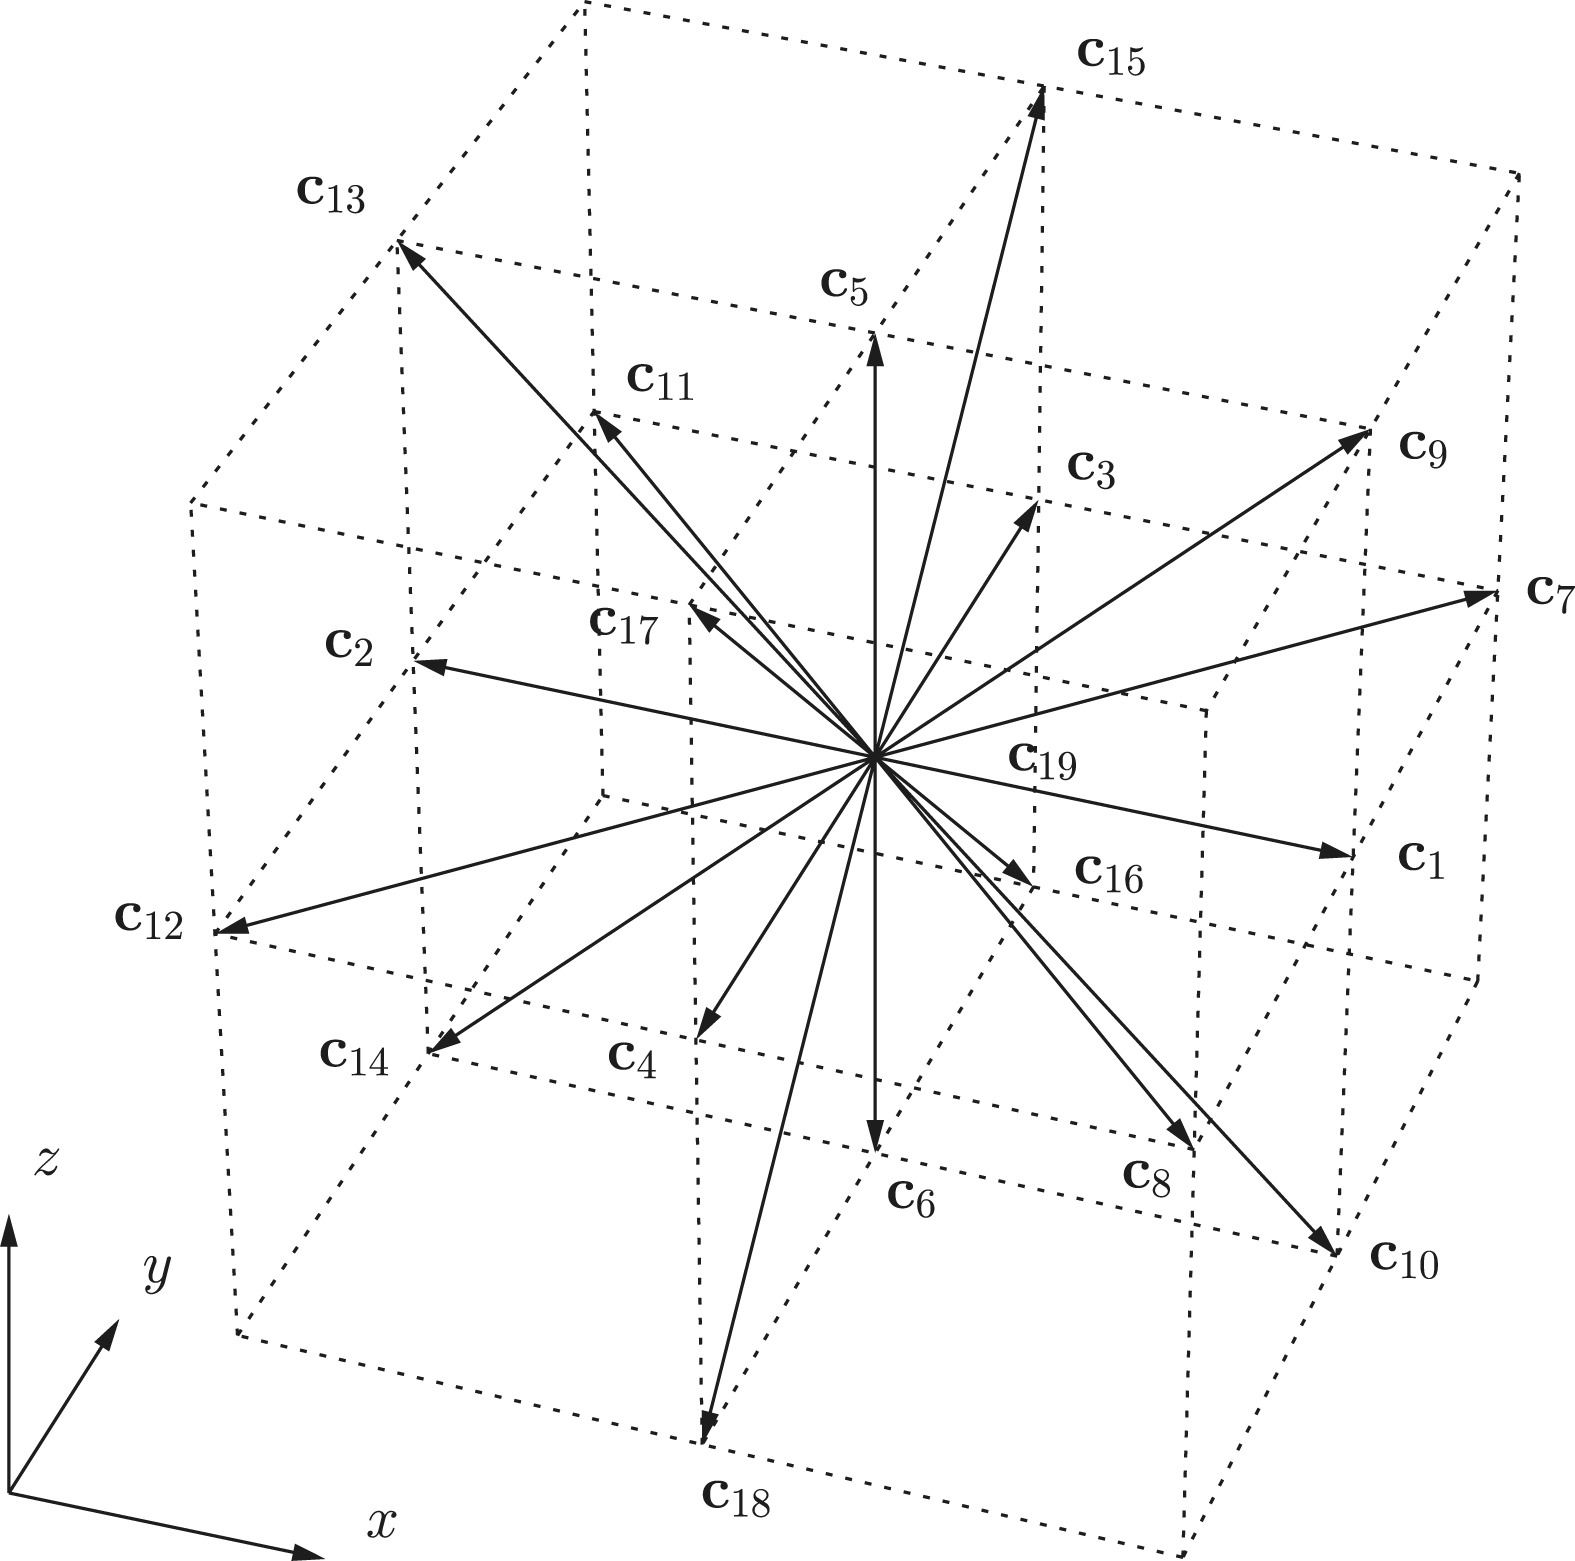
\includegraphics[scale = 1]{figures/methods/d3q19_lattice.jpg}
    \caption{D3Q19 lattice demonstrating the rest, nearest and next nearest direction that correspond to the 19 
    directions $(i)$ of the lattice with lattice velocity $c_{i}$. \cite{schmieschek_lb3d_2017} Reproduced from 
    Schmieschek et al. Computer Physics Communications 2017, 217, 149--161, under the Creative Commons license.}
    \label{fig:d3q19_lattice}
\end{figure}

The LBM is composed of a collision and advection step. In the advection step, the populations at each grid point are propagated to adjacent points in accordance 
with the chosen stencil. During the collision step, the particle population distribution is relaxed towards an equilibrium with a collision operator, at a 
specified relaxation rate. Importantly, LBM can be extended to handle multiphase and multicomponent fluids, using either color-gradient models, free energy formulations, 
or pseudopotential approaches to model non-ideal mixing. It also couples well to particle dynamics through momentum exchange schemes, making it a powerful framework for 
simulating colloidal suspensions, interfacial phenomena, and structurally complex systems like bijels. Its ability to capture both hydrodynamics and mesoscale thermodynamic 
behavior makes it particularly suited for the multi-scale requirements of stimuli-responsive emulsions.

In summary, the Volume of Fluid method offers robust interface tracking and mass conservation but lacks the ability to naturally capture interfacial curvature. 
Phase field methods provide thermodynamically consistent, diffuse-interface models ideal for phase separation, though they require fine resolution and are computationally intensive. 
Brownian dynamics excels at modeling particle-level stochastic motion but cannot resolve bulk fluid dynamics or interface evolution on its own. In contrast, the Lattice Boltzmann Method 
combines the strengths of mesoscopic fluid modeling with efficient handling of complex interfaces and straightforward coupling to particle dynamics. Its balance between computational 
efficiency, scalability, and physical fidelity across multiple scales makes LBM the most suitable method for simulating the rich interplay of hydrodynamics, phase separation, and particle 
interactions in stimuli-responsive emulsions such as bijels.

\subsection{Multicomponent models in the Lattice Boltzmann Method}

Four primary techniques exist in the lattice Boltzmann literature for modeling multicomponent or multiphase systems. These are the Shan-Chen (SC) 
pseudopotential model, the free energy (FE) model, the color gradient (CG) model, and the interface tracking (IT) model.
These methods differ fundamentally in their formulation and implementation, each offering unique advantages and trade-offs in terms of accuracy, 
stability, physical realism, and computational cost. Below, each approach is briefly reviewed, followed by a comparative discussion of their 
suitability for modeling stimuli-responsive emulsions such as bijels.

The SC model introduces fluid-fluid interactions via a local, density-dependent force, enabling spontaneous phase separation and interface 
formation without requiring explicit interface tracking. 
\cite{shan_lattice_1993, shan_simulation_1994, shan_multicomponent_1995, jansen_bijels_2011,gunther_timescales_2014}
Its simplicity and computational efficiency have made it a widely used method. However,
in this formulation, surface tension is not an independently controllable parameter. An effective mass defined from the density of each component
in each lattice point is used in the force calculation, meaning that it indirectly determines the surface tension in addition to the interaction
strength parameter.

The FE model is derived from a square-gradient free energy functional, which modifies the equilibrium distribution to incorporate thermodynamic 
forces driving phase separation. \cite{swift_lattice_1996, kendon_inertial_2001, briant_lattice_2004} Like the SC model, it naturally produces interfaces and captures interfacial tension. Unlike the SC model, however, 
the FE model allows for explicit control of surface tension and interface thickness via the bulk free energy parameters. This thermodynamic 
consistency makes it attractive for modeling systems with diffuse interfaces. The thermodynamics of the system can also be modified through changing the free energy used.
\cite{swift_lattice_1996, briant_lattice_2004, kendon_inertial_2001}
A key limitation, however, is its difficulty handling fluids with high density ratios, which can reduce its applicability in more extreme multiphase scenarios.

The CG model assigns color labels to each fluid component and applies a recoloring step to enforce immiscibility and sharpen the interface 
between fluids. 
\cite{mora_optimal_2021, latva-kokko_static_2005, huang_study_2014, liu_multiphase_2016}
This recoloring step is responsible for generating interfacial tension and enables precise control over interfacial properties such 
as surface tension and width. The model has demonstrated success in soft matter systems where interfacial control is critical. However, implementing 
the recoloring algorithm introduces additional complexity and requires careful parameter tuning to ensure stability and numerical consistency. \cite{mora_optimal_2021}

The IT model employs level-set or front-tracking techniques to explicitly track the location of fluid interfaces by evolving a separate indicator 
function, commonly defined using a level set technique, alongside the LB solver. \cite{haghani_hassan_abadi_conservative_2018, liang_lattice_2023}
This method achieves high accuracy in resolving interface position and curvature, making it ideal for problems 
involving surface tension-driven flows or sharp interfacial features. However, it is computationally intensive as the indicator function must be implemented alongside
the LB solver. 

Given these trade-offs, the Shan-Chen pseudopotential model is chosen for this research due to its balance between physical realism and computational 
efficiency. \cite{jansen_bijels_2011,gunther_timescales_2014, gunther_lattice_2013, xie_direct_2017}
Its ability to capture phase separation, interface formation, and emergent domain morphology without requiring explicit interface 
tracking or complex coupling makes it suitable for simulating the large-scale dynamics of bijels. Moreover, its straightforward coupling to 
colloidal particles facilitates the inclusion of particle-fluid and particle-interface interactions central to the system being studied.

\section{Implementing the multicomponent Lattice Boltzmann Method} 
\label{section:lbm_hydrodynamics}

The lattice boltzmann method works by evolving a population distribution $f_{i}(\mathbf{x}, t)$ on a cubic lattice with 
timestep $\Delta t$ with lengthscale $\Delta x$. \cite{qian_lattice_1992, succi_lattice_2018, he_theory_1997} The D3Q19 
velocity set is used in this work with the indexes $i$ represent each of the 19 velocities and conserves mass and momentum 
to the second order. It can be seen in Figure \ref{fig:d3q19_lattice}. The algorithm is split into the 
collision step where the populations on each lattice grid cell is relaxed towards an equilibrium, followed by the 
advection step where populations in each velocity direction are propagated with velocity $\mathbf{c_i}$. 

% The collision step occurs using a single relaxation time Bhatnagar-Gross-Krook (BGK) collision operator at relaxation 
% rate $\tau$. \cite{bhatnagar_model_1954, qian_lattice_1992} 

% The collision operator can have multiple forms based on how many relaxation rates are used although the most common variant is the 
% Single Relaxation Time (SRT) collision operator, more commonly known as the Bhatnagar-Gross-Krook (BGK) collision operator. 
% \cite{bhatnagar_model_1954, qian_lattice_1992} 
% Owing to its stability in low Mach 
% and Reynolds numbers and simplicity of implementation, the BGK operator is often used in particle laden flow and soft matter simulations. 
% \cite{bhatnagar_model_1954} These limitations are present owing to the implicit link between the fluid properties and the relaxation rate, 
% and to ensure fluid incompressibility from an equation that intrinsically simulates a compressible fluid. To get over these 
% limitations, Two Relaxation Time (TRT) and Multiple Relaxation Time (MRT) operators also exist, expanding the possible application of the LBM to visco-elastic 
% flows and implementation of fluctuating hydrodynamics in the LBM. \cite{liu_simulation_2023, adhikari_fluctuating_2005} The combined collision and advection 
% LBM is expressed below in equation \ref{eq:LBM_BGK}

The collision step in the LBM is performed using the collision operator. It can take multiple forms depending on the number of
relaxation rates used. The most commonly used variant is the Single Relaxation Time (SRT) operator defined with the Bhatnagar-Gross-Krook (BGK) 
collision operator \cite{bhatnagar_model_1954, qian_lattice_1992}. The BGK model is easy to implement and works well enough in soft matter and
particle-laden flow simulations.

However the BGK operator controls all moments at a single relaxation rate which can induce numerical instabilities and inaccuracies
at higher fluid velocities. \cite{liu_simulation_2023, adhikari_fluctuating_2005} These numerical instabilities can be resolved by using
a Multiple Relaxation Time (MRT) collision operator. However the relaxation rates used in an MRT collision operator must be tuned carefully
to ensure that the appropriate fluid properties are modelled. Simpler variants of the MRT collision operator such as the Two Relaxation Time (TRT)
collision operator have been proposed as a solution that provides some of the benefits of MRT models with the simplicity of SRT models. These 
have facilitated simulation of a wider range of physical phenomena \cite{adhikari_fluctuating_2005, liu_simulation_2023}. The SRT collision 
operator is selected due to the additional computational performance needed by MRT not being needed. The combined streaming and 
collision step in LBM, using the BGK operator, is expressed in Equation \ref{eq:LBM_BGK}.

\begin{equation}
    f_{i}(\mathbf{x} + \mathbf{c}_{i}\Delta t, t + \Delta t) = f_{i}(\mathbf{x}, t) - \frac{1}{\tau}(f_{i}(\mathbf{x}, t) 
    - f_{i}^{eq}(\mathbf{x}, t))
    \label{eq:LBM_BGK}
\end{equation}

The BGK operator limits simulations to low reynolds number and mach numbers to prevent numerical instabilities. 
\cite{qian_lattice_1992} The kinematic viscosity if using the BGK operator is defined as 
$\nu = c_s^2(\tau - \frac{\Delta t}{2})$. The equilibrium distribution is obtained from a taylor expansion of the 
Maxwell-Boltzmann distribution to the second order. \cite{he_theory_1997, succi_lattice_2018} This is shown in equation 
\ref{eq:LBM_Feq}.

\begin{equation}
    f_{i}^{eq}(\mathbf{x}, t) = w_i\rho(1 + \frac{\mathbf{c_i} \cdot \mathbf{u}}{c_s^2} + \frac{(\mathbf{c_i} \cdot 
    \mathbf{u})^2}{2c_s^4} + \frac{\mathbf{u} \cdot \mathbf{u}}{2c_s^2})
    \label{eq:LBM_Feq}
\end{equation}

$\rho$ and $\textbf{u}$ in Equation \ref{eq:LBM_Feq} are defined as the macroscopic parameters for density and velocity 
and can be calculated from the mass distribution using $\rho = \sum f_i$ and $\rho \mathbf{u} = \sum f_i \mathbf{c}_i$ 
respectively. Using the Chapman-Enskog expansion, the Navier-Stokes equation at the incompressible limit at low mach
numbers can be recovered. \cite{qian_lattice_1992, he_lattice_1997} The regime accessible through this method is suitable 
for simulations in this work as the $ 1 \leq Re \leq 100 $ and the mach number, $Ma < 0.01$, fulfilling the stability 
criterion and usage requirements for the presented hydrodynamic model.

The density and velocity of the fluid at each grid point is calculated from the zeroth and first moment of the particle density
distribution, 

\begin{equation}
    \begin{split}
        \rho &= \sum_i f_i \\
        \rho\vec{u} &= \sum_i f_i \mathbf{c_i}
    \end{split}
\end{equation}

The momentum flux tensor is calculated from the Chapman-Enskog expansion of \ref{eq:LBM_BGK} to the first order yielding,

\begin{equation}
    \begin{split}
        \rho\frac{\partial \vec{v}}{\partial t} + \nabla \cdot \Pi &= 0 \\
        \Pi_{\alpha \beta} &= \sum_i \mathbf{c_i}_\alpha \mathbf{c_i}_\beta (f_i^{eq} + (1 - \frac{1}{2 \tau})f_i^1)
    \end{split}
\end{equation}

The momentum flux tensor can be further expressed as a function of macroscopic variables, 

\begin{equation}
    \begin{split}
        \Pi^{(0)}_{\alpha \beta} &= \sum_i \mathbf{c_i}_\alpha \mathbf{c_i}_\beta f_i^{eq} = p \delta_{\alpha \beta} + \rho \vec{u}_\alpha \vec{u}_\beta \\
        \Pi^{(1)}_{\alpha \beta} &= (1 - \frac{1}{2 \tau})\sum_i \mathbf{c_i}_\alpha \mathbf{c_i}_\beta f_i^{eq} = \nu (\nabla_{\alpha}(\rho \vec{\beta}) + \nabla_{\beta}(\rho \vec{\alpha}))
    \end{split}
\end{equation}

With $p = \rho c_s^2$ and $\delta_{\alpha \beta}$ the kronecker delta.

\subsection{Non-ideal mixing}
\label{section:lbm_non_ideal_mixing}

The SC model mimics Cahn-Hilliard type behaviour through a force applied from the other fluid species $k'$ in adjacent 
cells $\mathbf{x'}$ on fluid species $k$ at point $\mathbf{x}$. \cite{shan_lattice_1993, shan_simulation_1994, 
shan_multicomponent_1995, he_discrete_1998, jansen_bijels_2011, chin_lattice_2002} Both fluid species are defined
by their own distribution equation defined in Equation \ref{eq:LBM_BGK} The strength of this force is controlled 
through an interaction parameter, $g_{kk'}$ with no contribution from self interaction of the fluid as these are 
set to zero. The SC force can then be written out in Equation \ref{eq:sc_model}.

\begin{equation}
% F_{k}^{SC}(\mathbf{x}, t) = -\Psi^{k}(\mathbf{x}, t)\sum_{k'}g_{cc'}\sum_{\mathbf{x'}}\Psi_{k'}(\mathbf{x'}, t)(\mathbf{x'} 
% - \mathbf{x})
\vec{F}_k(\vec{x}) \Delta t = - \sum_{k'} \sum_i \frac{w_i}{c_s^2} g_{kk'} \psi_k(\vec{x})\psi_{k'}(\vec{x}+\vec{c}_i) \vec{c}_i
\label{eq:sc_model}
\end{equation}

An effective mass of each fluid at node $\mathbf{x}$ is used in place of the actual density to scale it between zero 
and one and is defined as $\psi^{k}(\mathbf{x},t) = \rho_{0}\left[1 - \exp(-\frac{\rho^{k}(\mathbf{x}, t)}{\rho_{0}})\right]$. 
In this model, the SC force is incorporated into the macroscopic velocities that are then used to calculate the equilibrium
distribution $f_{i}^{k, eq}$ for fluid $k$, defined as,

\begin{equation}
\vec{u}_k^{\text{eq}} = \vec{u}' + \frac{\tau_k}{\rho_k} \vec{F}_k
\end{equation}

Where $\vec{u}'$ is defined as the common grid velocity and is calculated from $f_i^k$ below

\begin{equation}
    \sum_k \frac{\rho_k}{\tau_k} \vec{u}' = \sum_k \frac{1}{\tau_k}\sum_i f_i^k\vec{c}_i
\end{equation}

This recasting of the velocity ensures that in the absence of forces, the total momentum of the system is conserved. 

% \textcolor{blue}{https://doi.org/10.1103/PhysRevE.84.046710}

\subsection{Suspended particle dynamics}
\label{section:lbm_colloids}

Suspended particles will be coupled to the LB fluid based on the work conducted by Ladd. \cite{ladd_numerical_1994, 
aidun_direct_1998, ladd_lattice-boltzmann_2001} The particles follow Newtonian mechanics with the particle force and
rotational inertia defined using differential equations

\begin{equation}
    \begin{split}
    \vec{F_p} = m_p \frac{\vec{u}_p}{dt} , \\
    \vec{D_p} = \mathbf{J}_p \frac{\vec{\omega}_p}{dt} ,
    \label{eq:md}
    \end{split}
\end{equation}

$\mathbf{F_p}$ and $\mathbf{D_p}$ represent the force and torque acting on a particle with mass $m_p$ and moment of inertia 
$\mathbf{J}_p$. $\mathbf{u}_p$ and $\mathbf{\omega_{p}}$ are the linear and angular velocities of the particle. The equations of 
motion are evolved over time using a leapfrog integrator. \cite{jansen_bijels_2011}

The particles are discretized on the lattice according to the method laid out in Ladd and Aidun 
\cite{ladd_lattice-boltzmann_2001}. Nodes representing the particle are marked as solid nodes that replicate
a no-slip boundary condition through a moving bounce-back boundary. This is implemented into the distribution function
by reflecting the outgoing populations of $f_i^k$ to the opposite lattice velocity

\begin{equation}
    f^k_{i^\star}(\vec{x}, t+\Delta t) = f^{k,\star}_i(\vec{x}, t) - \frac{2w_i}{c_s^2} \rho \vec{u}_i \cdot \vec{c}_i ,
\end{equation}

This facilitates momentum exchange between particle and fluid which can be calculated analytically as 
\(\Delta\vec{p}^k_i \frac{\Delta t}{(\Delta x)^3} = 2 f^{k,\star}_i(\vec{x},t)\vec{c}_i - \frac{2w_i}{c_s^2}\rho(\vec{u}_i\cdot\vec{c}_i)\vec{c}_i\).
The sum of the momentum change across the surface of the particle is computed to obtain the force and torque on the particle,

\begin{equation}
    \begin{split}
    \vec{F}_p &= \sum_{k,i} \frac{\Delta \vec{p}^k_i}{\Delta t} , \\
    \vec{T}_p &= \sum_{k,i} \frac{\Delta\vec{p}^k_i}{\Delta t} \times \vec{r}_i .
    \end{split}
\end{equation}

As the particle moves, the nodes representing the particle are updated, with newly covered grid points marked as solid and 
uncovered nodes marked as fluid. When a grid point is covered, the momentum contained in that lattice point is added to the 
total force of the particle,

\begin{equation}
    \vec{F}_p = -\sum_{k,i} f_i^k(\vec{x},t)\vec{c}_i .
\end{equation}

Upon uncovering of a grid point, it is assigned a density value that represents the average of all adjacent fluid sites,

\begin{equation}
    \rho^k(\vec{x},t) = \frac{1}{N_{\text{f}}} \sum_{i_{\text{f}}} \rho^k(\vec{x}+\vec{c}_{i_{\text{f}}n}, t)
    \label{eq:fill_particles}
\end{equation}

\subsubsection{Anisotropic particles}
\label{section:lbm_colloids_ellipsoids}

For particles close to contact, meaning with inter-surface distances under 1 lattice unit the hydrodynamics are unresolved as the
distance is smaller than what the model can resolve. Lubrication forces are added to reduce the likelihood of particle overlap. For 
spherical particles, this is defined in Equation \eqref{eq:lubrication}

\begin{equation}
    \vec{F}_l = -6 \pi \eta \frac{R_1^2 R_2^2}{\left(R_1+R_2\right)^2}\left(\frac{1}{|\vec{r}_{ij}|-R_1-R_2}-\frac{1}{d_c}\right) \frac{\left(\vec{u}_{12}\cdot\vec{r}_{12}\right)\vec{r}_{12}}{|\vec{r}_{12}|^2} ,% \qquad d<d_c,
    \label{eq:lubrication}
\end{equation}

where $R_i$ and $R_j$ are the radii of each particle involved in the interaction, $\vec{r}_{ij}$ is the distance
vector between the particle centers, $\mathbf{u}_{ij}$ are the relative velocities of the particles and $\Delta_c$ 
is the cutoff distance when the lubrication force begins to act. If particles are able to overcome the lubrication forces, 
a hertzian contact force is also added to ensure that there is no particle overlap, defined in Equation \eqref{eq:hertz}

\begin{equation}
    \phi_{H} = K_{H}(R_i + R_j - |\mathbf{r}_{ij}|)^{5/2}, r < R_i + R_j
    \label{eq:hertz}
\end{equation}

$K_H$ is the force constant used to push particles apart. To correct for the anisotropic particles used in this work, 
the formulas presented in Eqs \ref{eq:lubrication} and \ref{eq:hertz} can be generalized using the route followed 
in Gunther et al. and Davies et al., inspired by Berne and Pechukas. \cite{gunther_timescales_2014, davies_interface_2014} 
They first begin by rewriting the lubrication and Hertzian contact forces as a function of the particle orientation and 
aspect ratio of the particles.

\begin{equation}
    \begin{split}
    \phi(\vec{r}_{ij}) &= {\epsilon} \tilde{\phi}\left(\frac{\vec{r}_{ij}}{{\sigma}}\right) , \\
    \vec{F}(\vec{r}_{ij}) &= {\epsilon} \tilde{\vec{F}}\left(\frac{\vec{r}_{ij}}{{\sigma}}\right) .
    \end{split}
\end{equation}

For the lubrication force \eqref{eq:lubrication}, we choose
${\sigma}=R_1+R_2$ and ${\epsilon}=\frac{6\pi\eta R_1^2 R_2^2}{{\sigma^3}}$, and for the
Hertz potential we chose ${\sigma}=R_1+R_2$ and ${\epsilon}=K_H\sigma^{5/2}$. For two identical, rotationally
symmetric ellipsoidal particles with orientations $\hat{\vec{o}}_i$ and $\hat{\vec{o}}_j$, we then replace $\epsilon$ and $\sigma$ by
the anisotropic functions

\begin{equation}
    \begin{split}
    \tilde\epsilon\left(\hat{\vec{o}}_i, \hat{\vec{o}}_j\right) &= \frac{{\epsilon}}{\sqrt{1-\chi^2}} , \\
    %\qquad \chi = \frac{\left(\alpha^2-1\right)R_\parallel^2}{\left(\alpha^2+1\right)R_\parallel^2}\left(\hat{\vec{o}}_i\hat{\vec{o}}_j\right) , \\
    \tilde\sigma\left(\vec{r}_{ij}, \hat{\vec{o}}_i, \hat{\vec{o}}_j\right) &= \frac{{\sigma}}{\sqrt{1-\frac{\chi}{2}\left[ \frac{\left(\hat{\vec{r}}_{ij}\cdot\hat{\vec{o}}_i+\hat{\vec{r}}_{ij}\cdot\hat{\vec{o}}_j\right)^2}{1+\chi\left(\hat{\vec{o}}_i\hat{\vec{o}}_j\right)} + \frac{\left(\hat{\vec{r}}_{ij}\cdot\hat{\vec{o}}_i-\hat{\vec{r}}_{ij}\cdot\hat{\vec{o}}_j\right)^2}{1-\chi\left(\hat{\vec{o}}_i\hat{\vec{o}}_j\right)} \right] }} , \\
    \chi &= \frac{\alpha^2-1}{\alpha^2+1} , \\
    \end{split}
\end{equation}

where $R_{\parallel}$ is the particle radius along the
symmetry axis $\hat{o}$ and $\alpha=\frac{R_{\parallel}}{R_{\perp}}$ the aspect
ratio of the particle. The anisotropic Hertz potential and lubrication
force are then defined as
%
\begin{equation}
    \begin{split}
    \phi\left(\vec{r}_{ij}, \hat{\vec{o}}_i, \hat{\vec{o}}_j\right) &= \epsilon\left(\hat{\vec{o}}_i, \hat{\vec{o}}_j\right) \tilde{\phi}\left(\frac{\vec{r}_{ij}}{\sigma\left(\vec{r}_{ij}, \hat{\vec{o}}_i, \hat{\vec{o}}_j\right)} \right) , \\
    \vec{F}\left(\vec{r}_{ij}, \hat{\vec{o}}_i, \hat{\vec{o}}_j\right) &= \epsilon\left(\hat{\vec{o}}_i, \hat{\vec{o}}_j\right) \tilde{\vec{F}}\left(\frac{\vec{r}_{ij}}{\sigma\left(\vec{r}_{ij}, \hat{\vec{o}}_i, \hat{\vec{o}}_j\right)} \right) .
    \end{split}
\end{equation}

\subsection{Magnetic field and particle coupling}
\label{section:lbm_colloids_magnetics}

The magnetic dipole potential is defined as

\begin{equation}
    \mathbf{U_{ij}} = \frac{\mu_0 m_i m_j}{4\pi r_{ij}^{3}} \left[ \Hat{\mathbf{o_i}} \cdot \Hat{\mathbf{o_j}} - 
    3(\Hat{\mathbf{o_i}} \cdot \Hat{\mathbf{r_{ij}}})(\Hat{\mathbf{o_j}} \cdot \Hat{\mathbf{r_{ij}}}) \right]
    \label{eq:magnet_potential}
\end{equation}

Where $\mu_0 = 4\pi \cdot 10^{-7} \frac{H}{m}$,  $\Hat{\mathbf{o_i}}$ is the orientation unit vector of particle 
$i$, $\Hat{\mathbf{r_{ij}}}$ is the distance vector between particles $i$ and $j$ and $m_i$ is the magnitude the 
magnetic dipole of particle $i$. From the potential, the force and torque of the dipole force between particles 
can be found. These expressions are shown in equations \ref{eq:dipole_magnetic_force} and \ref{eq:dipole_magnetic_torque} 
for the force and torque respectively.

\begin{equation}
    \mathbf{F}_{ij} = \frac{3 \mu_0}{4 \pi} [\frac{5(m_i \cdot \mathbf{r}_{ij})(m_j 
    \cdot \mathbf{r}_{ij})}{|\mathbf{r}_{ij}|^7}\mathbf{r}_{ij} - \frac{(m_i \cdot m_{j})\mathbf{r}_{ij} + 
    (m_i \cdot \mathbf{r}_{ij})m_i + (m_j \cdot \mathbf{r}_{ij})m_j }{|\mathbf{r}_{ij}|^5}]
\label{eq:dipole_magnetic_force}
\end{equation}

\begin{equation}
    \mathbf{T}_{ij} = \frac{\mu_0}{4 \pi}[ \frac{3(m_j \cdot \mathbf{r}_{ij})m_i \times \mathbf{r}_{ij} }
    {|\mathbf{r}_{ij}|^5} - \frac{m_i \cdot m_j }{|\mathbf{r}_{ij}|^3} ]
    \label{eq:dipole_magnetic_torque}
\end{equation}

Equations \ref{eq:magnet_force} and \ref{eq:magnet_torque} are used to calculate the force and torque that the 
field exerts on each particle.

\begin{equation}
    \mathbf{F_{j}} = (m_j \Hat{\mathbf{o_j}} \cdot \nabla B_i)
    \label{eq:magnet_force}
\end{equation}

\begin{equation}
    \mathbf{\tau_j} = (m_j \Hat{\mathbf{o_j}} \times B_i)
    \label{eq:magnet_torque}
\end{equation}

The total force and torque exerted on each particle is the sum of the particle dipole interaction and the field 
dependent contribution. 